\chapter{Introduction}
\thispagestyle{fancy} Le but de ce projet était de nous familiariser
avec les environnement 3D et de faire une première approche des
systèmes multi-agents. Le cadre était de créé deux types d'agent, l'un
devant ammasser des pierres pour construire un chateau, l'autre devant
empecher les premiers de le faire. Le moteur 3D utilisé était le
moteur open source Ogre utilisé avec sa surcouche C\#, Mogre.

Nous avons simulé deux types d'agents ; un agent représenté par un ninja qui a comportement constructeur et un agent représenté par un robot qui a un comportement destructeur. Les agent détruise ou construise des tas de pierre symbolisé par des têtes d'ogre.
\\
\begin{center}
\begin{tabular}{c c}
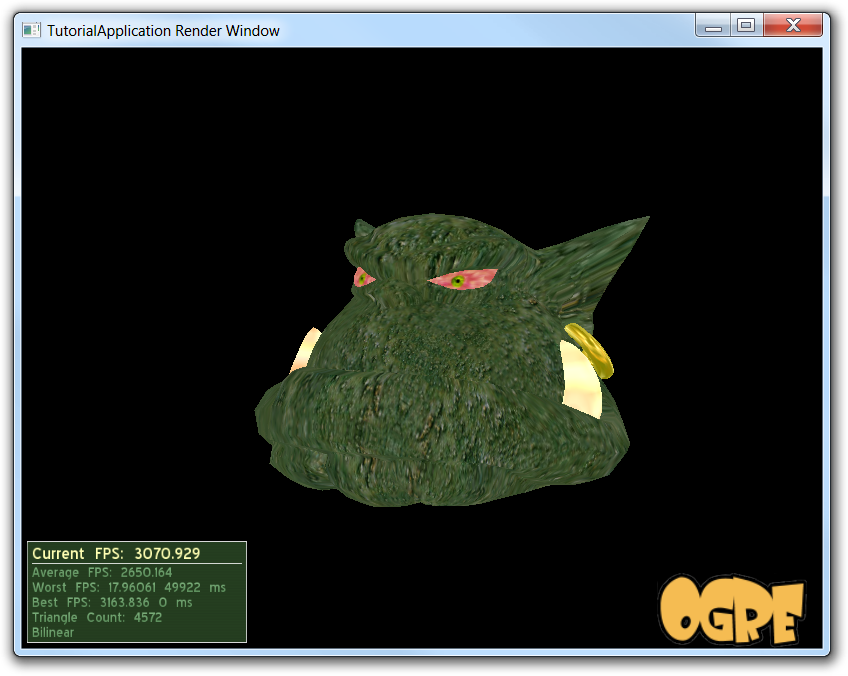
\includegraphics[width=7cm]{Images/mogre_logo.png}
&
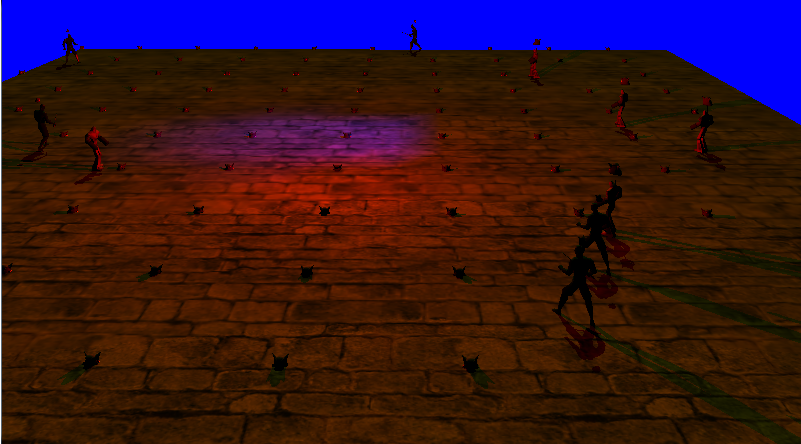
\includegraphics[width=8cm]{Images/mogre_capture.png}
\end{tabular}
\end{center}
